\chapter{FlipIt game with virus propagation}
\label{chapter2:FlipIt with virus propagation}
%\documentclass[10pt]{article}
%\begin{document}

%%%%%%%%%%%%%%%%%%%%%%%%%%%%%%%%%%%%%%%%%%%%%%%%%%%%%%%%%%
%%%%%			Introduction Chapter 1				%%%%%%
%%%%%												%%%%%%
%%%%%												%%%%%%
%%%%%%%%%%%%%%%%%%%%%%%%%%%%%%%%%%%%%%%%%%%%%%%%%%%%%%%%%%

\section{Introduction}
\label{Ch2:Intro}
The game of FlipIt with virus propagation considers attackers where their moves are not instantaneous. This can be motivated by an example of a virus. A virus can be dropped on a network but it only compromises the whole network if every node in the network is infected. The basic FlipIt game does not take this into account. In this chapter the FlipIt game with virus propagation is explained and how it can be modelled. First the main differences with the basic FlipIt game are discussed in section \ref{ch2:diffFlip}. Next in section \ref{ch2:formal} the formal definition of the game with virus propagation is given. At last, in section \ref{ch2:periodicvirus} a periodic strategy game is considered and the formalization of the formulas with virus propagation are determined.\\

This chapter explains how to model a FlipIt game with a virus propagation that infects a network. The first section explains the difference between a normal FlipIt game and a FlipIt game with virus propagation. The next section derives a formula to calculate the benefit for a FlipIt game with a virus propagation. In the last section we calculate the Nash equilibrium for the benefit formula.
\section{FlipIt game with virus propagation}

Motivation

\section{Explaining difference between FlipIt with and without virus propagation}
\label{ch2:diffFlip}
\begin{figure}[hbtp]
\caption{The first game is the basic FlipIt game. The second is a FlipIt game with a delay. During the first flip of the attacker, the defender moves after the delay, causing the attacker to get control over the resource. During the second flip of the attacker, the defender flips at time t+d, causing the defender to take control over the resource before the attacker. During the third and final flip of the attacker, the defender flips during time t+d, causing the attacker to never gain control over the resource. }
\centering
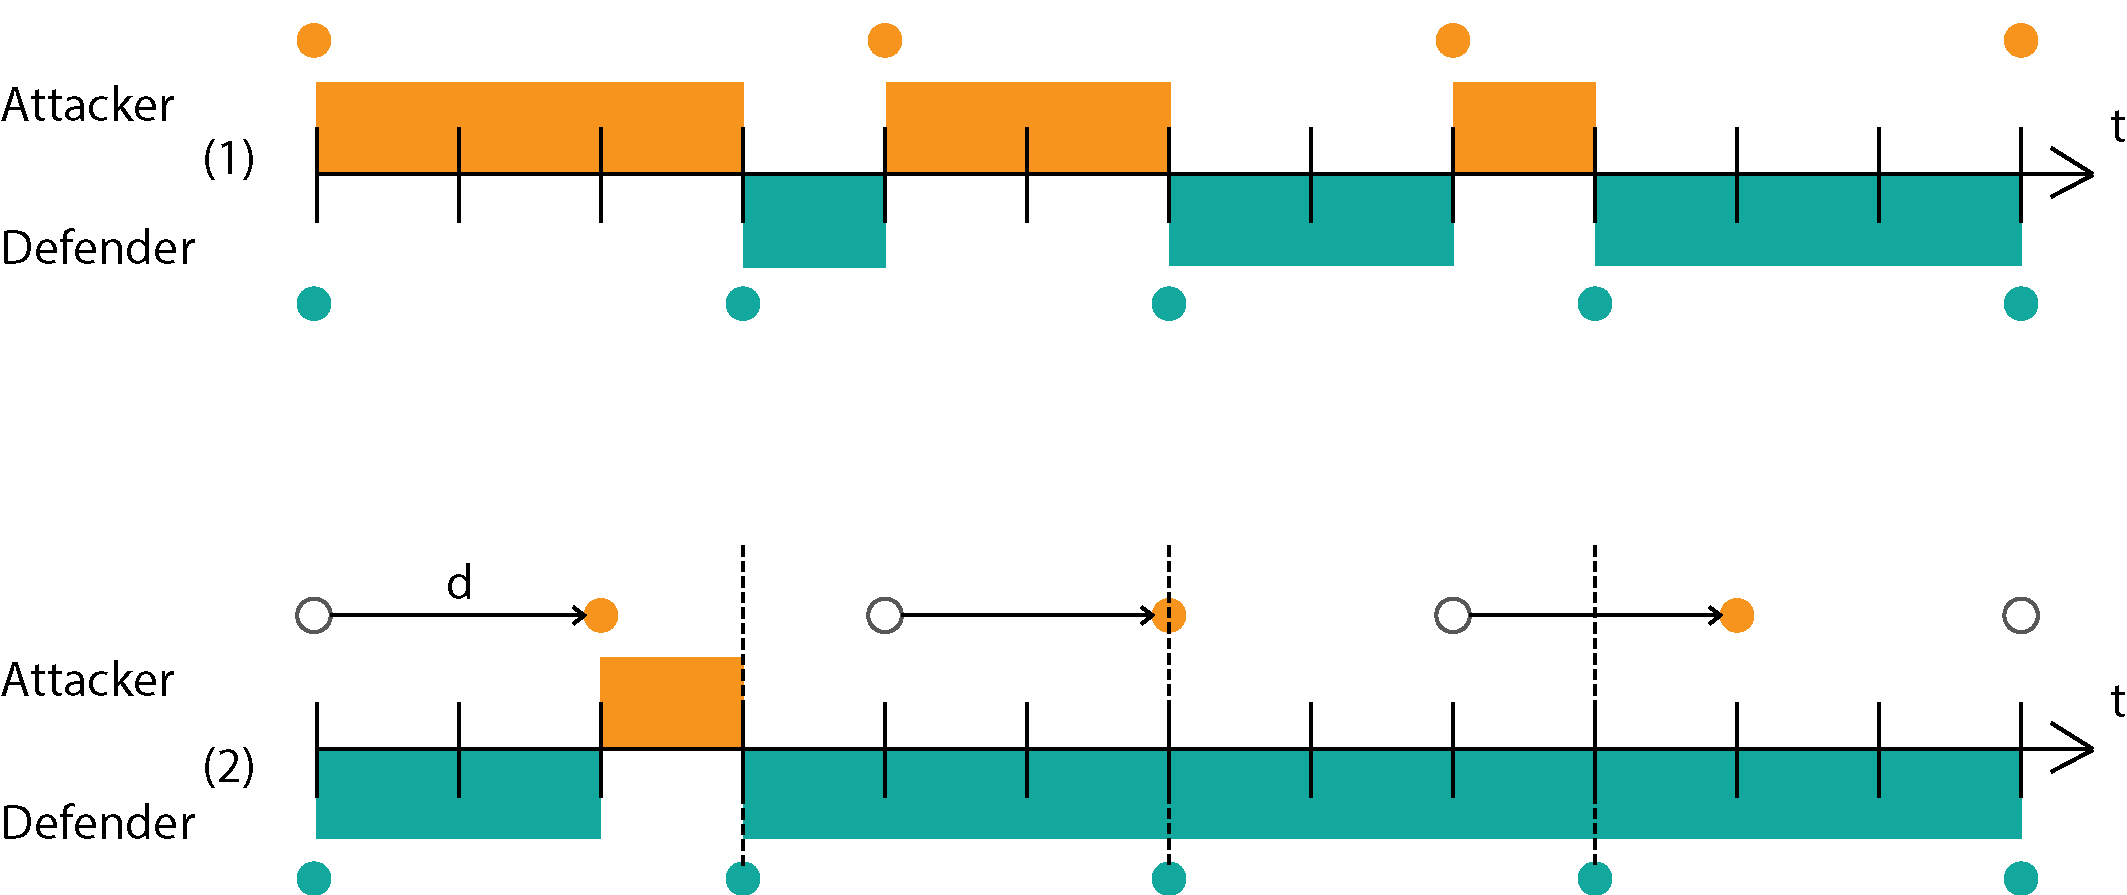
\includegraphics[scale=0.7]{Images/dtFlip.png}
\label{dt}
\end{figure}

A FlipIt game consists of a single resource. To represent the security problem, the game now defines its single resource as a computer network with multiple
nodes. One of the players, the defender, will try to defend his network. The defender
will do this by flipping all the nodes of the network (i.e. the entire resource) in every move he plays. The
attacker on the other hand will try to infect all the nodes in the network. The attacker
will do this by flipping the node in the graph that can infect all the nodes in the
shortest possible time. After dropping a virus on the first node, it takes a while for the virus to infect the entire network. Since the original FlipIt game works with a single resource that is always flipped entirely, the assumption is made that the attacker is considered to gain immediate full control over the resource when the network has been infected, even it is only one node that has been infected.\\

In reality however, after dropping a virus on the first node, it takes a while for the virus to infect
the entire network. So, the assumption that the attacker has full control over the resource as soon as a node has been infected, is not realistic. The attacker has only control of the network once all or a sufficient number of nodes are infected. 
The time that it takes for the virus to infect every node (or a sufficient number of nodes) will be
denoted as an infection-delay variable \textit{d} (called 'delay' for short in the remainder of this paper). If we want to measure how long it takes for the virus to
infect all the nodes in the network, we have to calculate the shortest path from the
first infected node to the farthest node. Rather than denoting the time needed for infecting \textit{all} the nodes, the variable $d$ can also be used to denote the time needed to infect \textit{a sufficient number} of nodes.

Assume that an attacker attacks at time \textit{t}, he doesn't get immediate control over the resource, but he only gains control at time \textit{t + d}, with $d$ denoting the time needed to infect a sufficiently number (or all) nodes. If the defender flips the network before the period $d$ has elapsed (so, somewhere between $t$ and $t + d$), then the attacker will never gain full control over the resource. See figure \ref{dt}. This implies that the mathematical formulas for gain and benefit need to be adapted to the fact that the attacker loses part of its benefit because of this delay. In the remainder of this paper, we will adapt the formalization of the FlipIt game using the variable $d$. \\ 


%%------------------------------------------------%
%%            Intro Game Theory 					 %
%%------------------------------------------------%
%\subsection{Actions of the attacker}
%A virus has different kind of ways of making his way through a company network. We will describe the different ways of how the virus can propagate. For start we will say that the virus or worm will be dropped on Node i and that it has k numbers of neighbours. 
%\begin{enumerate}
%\item Node i is infected and will spread the virus or worm to every k neighbours and will stop infecting the neighbours in the next step
%\item Node i is infected and will spread the virus or worm to every k neighbours and will keep on spreading the virus to the same neighbours in every next step
%\item Node i is infected and will spread the virus to only one of the k neighbours and will stop infecting another neighbour in the next step
%\item Node i is infected and will spread the virus to only one of the k neighbours and in the next step it will infect another one of the k neighbours 
%\end{enumerate}
%
%In the game that will be modelled in the paper we will use the settings of the first spreading method. We will not use method 2 because this kind of propagation will float the network. Because we use the settings of a mail system and contact in a mailing list the method of 3 and 4 are not used. \\
%In the first method the node that has been infected can be again infected. If one of the neighbours infects the node again the node will infect his neighbours again. By using this spreading method we have three distinct states in which a node can be situated. An \textit{infected state}, a \textit{clean state} and a \textit{spreading state}. An infected state means that the node is infected and will not spread the virus to its neighbours, a clean state means that the node is not infected on that moment and a spreading state means that the node is infected and that it will spread the virus or worm to its neighbours in the next step.
%We can argument this kind of propagation through a mail worm. \todo{voorbeeld geven van zo een worm}
%%Another propagation method is that the virus works as a token. It will propagate to only one neighbour and continue to spread. 
%
%The Attacker itself has two different ways of attacking the company network. It will only infected one node of the network and will wait for the virus to spread itself through the network. We will model two ways of attacks of an Attacker:
%\begin{enumerate}
%\item The attacker drops the virus on a random node on the network
%\item The attacker drops the virus on a targeted node on the network
%\end{enumerate}
%The attacker in this game will put a virus or worm on one of the nodes in the network. (This will happen at random.) The attacker does not know on which node the virus will be dropped. We will use this randomness because \todo{feit uit security rapport symantec} most viruses are spread via a usb stick or a shared resource. If we use this spreading method where we have a targeted attack the attacker will have more information about the network. \\
%
%The attacker can choose at which rate it will drop a virus on one of the nodes on the network. The cost of dropping a virus will be the same. It will not increase. If it will increase this means that the attacker will eventually drop out of the game because it becomes to expensive.\\
%The attacker is in control over the game if it manages to infect a subset of all the resources of the company network.
%
%
%\subsection{Actions of the defender}
%The attacker wants to protect all the nodes of his network. It can do so by getting back control over the resources. We will assume that the defender of the network has knowledge over his own network. Which is convenient in the real world because a company has to know how his infrastructure looks like.\\
%
%The defender has two possible ways of defending its network:
%\begin{enumerate}
%\item The defender flips all the nodes of his network
%\item The defender will flip a subset of the nodes of his network
%\end{enumerate}
%
%The cost of flipping all the nods of the network will be greater than the cost of flipping a subset of nodes. We make this assumption because otherwise it will be beneficial for the defender to always flip all the nodes in the network.\\
%
%We will also make the assumption that as a defender flips a node the node can get infected again. A flip will not be  correlated to a patch but to a clean-up. \todo{waarom geen patch, wormen kunnen veranderen gaandeweg}
%\todo{andere mogelijkheid:} Another setting of the game can be that the flip of the defender is equal to a patch and that the resource cannot be infected any more. But with this case we deviate from the flipIt game, because the attacker cannot flip the resource any more. Unless we work with different virusses every time the attacker flips. We start with the less complex game of flipping is equal to a clean-up.




\section{Playing periodically with virus propagation}
\label{ch2:periodicvirus}




The formalization starts from the model of the non-adaptive continuous basic FlipIt game where players use a periodic strategy with a random phase. This choice is motivated by the assumption that in most organisations, the defence strategy is to periodically defend the network. This corresponds to a periodic defender strategy.  A periodic attacker strategy is assumed as well, to be able to compare the results with the periodic strategy of the FlipIt game in \cite{FlipIt}. %, as this also corresponds to a common real life strategy. %nog eventueel verder te motiveren
Further research can investigate the effect of relaxing this assumption. \\



Similarly as in \cite{FlipIt}, we split the formalization in two cases. The first case is where the defender plays at least as fast as the attacker, the second case is where the attacker plays at least as fast as the defender. For each of these cases, first the benefit formula of the basic case without delay is presented, and then the delay is introduced.  \\

Intuitively we could assume that $d$ can never be bigger than $\delta_{A}$ because then the benefit for the defender would always be 1. This is not always true. It is only true if $d$ is bigger than $\delta_{D}$, because then the defender will always be in control. For this we only calculate the formulas for the cases where $d$ is smaller than $\delta_{D}$. We can already conclude that it is no use for the attacker to play when the delay is bigger than $\delta_{D}$. \\

\subsection{Formalization the benefit formula including the infection-delay}



 A Periodic strategy is a non-adaptive renewal strategy where the time intervals between consecutive moves are a fixed period, denoted by $\delta$. Moreover it has a random phase, that is chosen uniformly and random in the interval $[0,\delta]$ for the first move. The average rate of play of a player is denoted by $\alpha_{i} = \dfrac{1}{\delta_{i}}$. List of symbols that will be used throughout the paper. Figure \ref{FlipItDelay} represents a couple of the symbols for clarification.\\
~~\\
\begin{figure}[hbtp]
\caption{Formalization of a FlipIt game with delay: A representation of a FlipIt game where both players are playing periodically. Every move or flip is indicated by a blue or orange circle.  The defender is represented in blue and plays with a period of $\delta_{D}$. The flip of the attacker is represented by a white circle, but because there is a delay d, the attacker only controls the resource after time d represented by an orange circle. The attacker plays with a period of $\delta_{A}$. The blue and orange rectangles represent the amount of time the respective player is in control of the resource.}
\centering
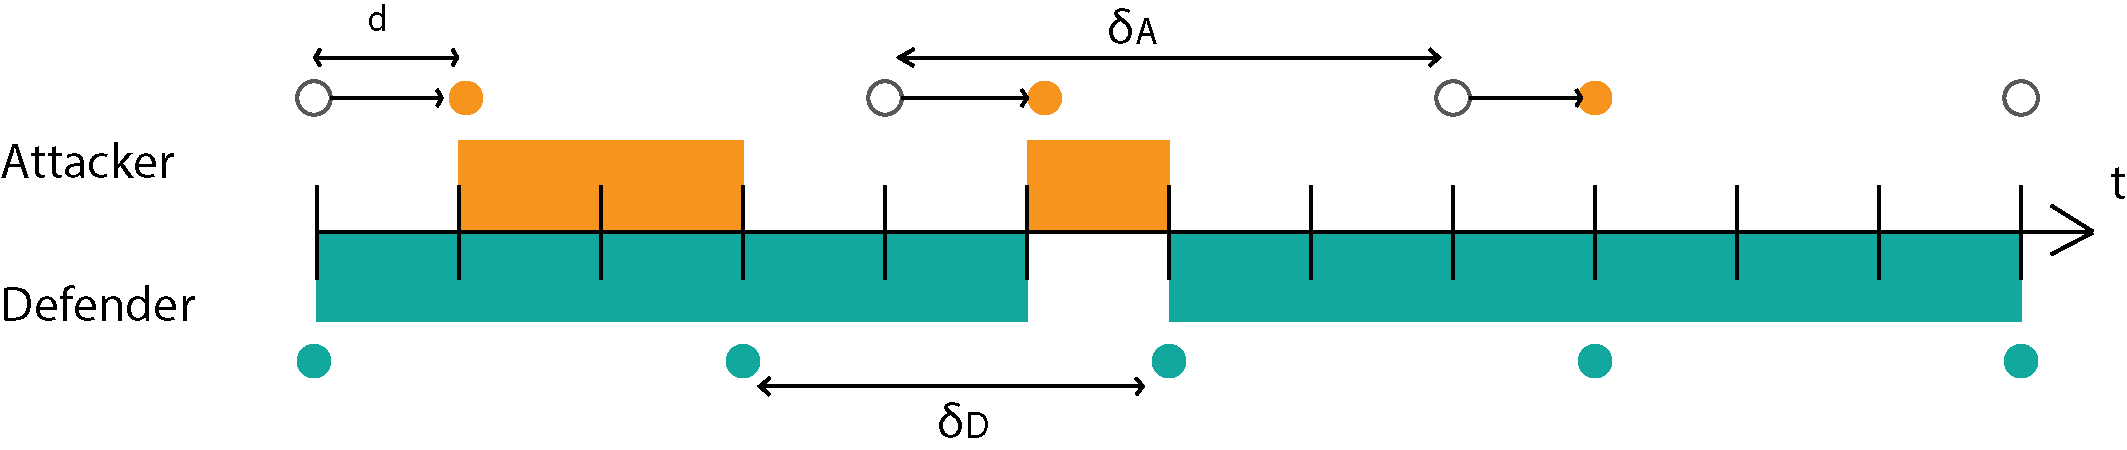
\includegraphics[scale=0.7]{Images/DefFlip.png}
\label{FlipItDelay}
\end{figure}

\begin{description}
\item $i$: Defines the player. Different as in the FlipIt paper where the defender is denoted by the subscript 0 and the attacker by the subscript 1.
\item $\delta_{i}$: The length of the interval between two consecutive moves of player \textit{i}. 
\item $\alpha_{i}$: The average flip rate of player \textit{i}, given by $\alpha_{i}=1/\delta_{i}$.
\item $k_{i}$: The cost of player \textit{i}'s moves.
\item $d$: The delay caused by the virus propagation.
\item $G_{i}(t)$: The total gain of player \textit{i} denotes the amount of time player \textit{i} is in control over the resource up to time \textit{t}.
\item $\gamma_{i}$: The average gain rate of player \textit{i} defined as $G_{i}(t)/t$
\item $\beta_{i}$:  The average benefit rate up to time \textit{t} defined as  $\beta_{i} = \gamma_{i} -k_{i} \alpha_{i} $.
\item $opt_{i}$: The optimum function.
\end{description}




\subsection*{\textbf{Case 1:} $\delta_{D} \leq \delta_{A} $ (The defender plays at least as fast as the attacker.) }

Let $r = \dfrac{\delta_{D}}{ \delta_{A} }$. The intervals between two consecutive defender's moves have length $\delta_{D}$. Consider a given defender move interval. The probability over the attacker's phase selection that the attacker moves in this interval is r. Given that the attacker moves within the interval, he moves exactly once within the interval (since $\delta_{D} \leq \delta_{A} $) and his move is distributed uniformly at random. \\

The expected period of attacker control within the interval would be r/2, without considering the delay by a virus. Therefore the benefit for the attacker, without considering the delay, can be expressed as follows:

\begin{equation*}
\beta_{A}(\alpha_{D},\alpha_{A}) =\dfrac {r} {2} - k_{A} \alpha_{A} = \dfrac {\delta_{D}} {2\delta_{A}} - k_{A} \alpha_{A}  
\end{equation*}\\

Correspondingly, the benefit for the defender can be expressed as:
\begin{equation*}
\beta_{D}(\alpha_{D},\alpha_{A}) =1 -  \dfrac {r} {2} - k_{D} \alpha_{D} = 1 - \dfrac {\delta_{D}} {2\delta_{A}} - k_{D} \alpha_{D} 
\end{equation*}

\begin{figure}[hbtp]
\caption{Case 1: Difference between a basic FlipIt game and a FlipIt game with a delay. (1) is the FlipIt game without a delay and (2) is with a delay. The delay is denoted with an arrow. The attacker is only in control when the circle becomes orange.}
\centering
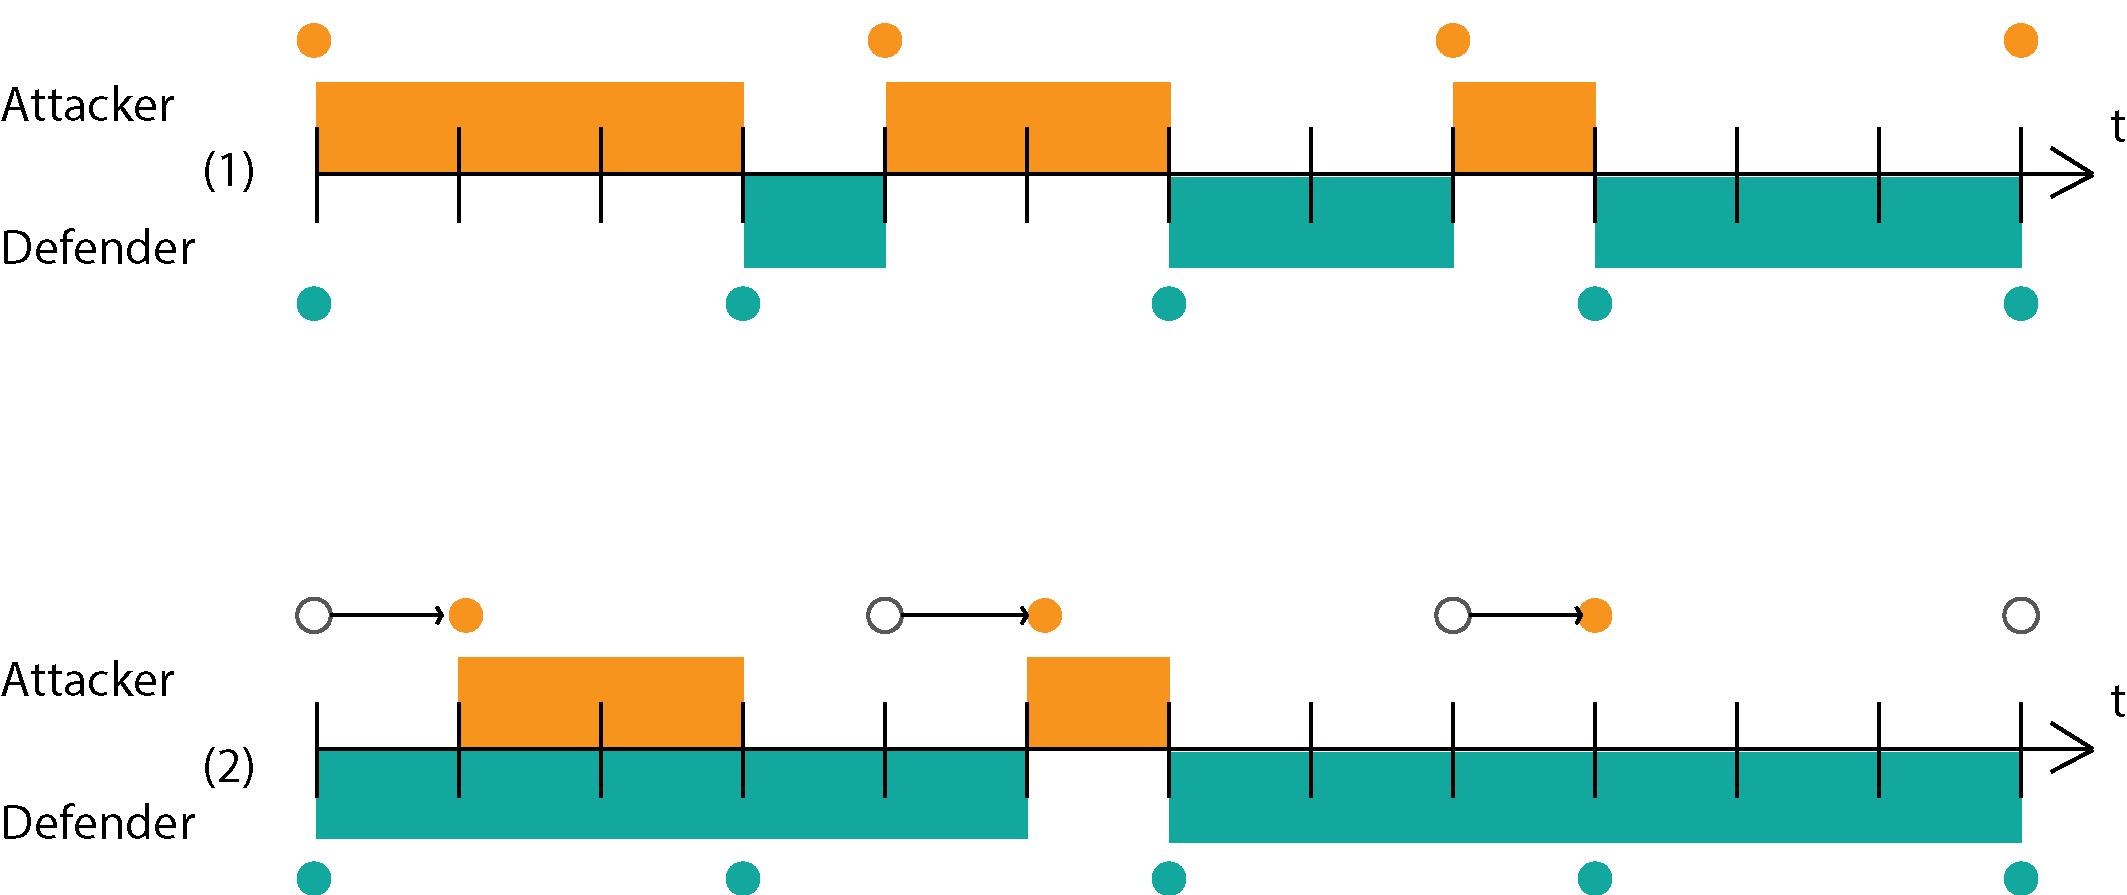
\includegraphics[scale=0.6]{../../doc/template/Images/DiffDelayCase1.png}
\label{fig:delaycase1}
\end{figure}


However, because of the delay required for virus propagation, the maximal time of control is reduced to $\delta_{D}-d$ , see figure \ref{fig:delaycase1}. There is a probability of \textit{r} that the attacker will move in the interval of the defender. However, the gain will not be half of the interval. Indeed, the attacker has to play soon enough to gain control, meaning that the attacker has to play during the period of $\delta_{D}-d$ during the interval of the defender. The probability that the attacker plays soon enough is $\dfrac{\delta_{D}-d}{\delta_{D}}$ and this will give the attacker an average gain of $\dfrac{\delta_{D}-d}{2}$. If the attacker moves after the period of $\delta_{D}-d$, the gain of the attacker will be zero. The probability that this happens is  $\dfrac{d}{\delta_{D}}$. The average gain rate of the attacker can then be expressed as follows if we look at one interval of the defender:
\begin{equation*}
\gamma_{A}(\alpha_{D},\alpha_{A}) = \dfrac {1}{\delta_{D}} [ \dfrac{\delta_{D}}{\delta_{A}} \cdot \dfrac{\delta_{D}-d}{\delta_{D}} \cdot \dfrac{\delta_{D}-d}{2} + \dfrac{\delta_{D}}{\delta_{A}} \cdot \dfrac{d}{\delta_{D}} \cdot 0 ]
\end{equation*}

To derive the benefit, the cost of moving is subtracted from the average gain. 
\begin{equation*}
\beta_{A}(\alpha_{D},\alpha_{A}) = \dfrac { (\delta_{D}-d) ^{2}} {2 \cdot \delta_{D}  \delta_{A}} - k_{A} \alpha_{A}
\end{equation*}
\begin{equation*}
\beta_{A}(\alpha_{D},\alpha_{A}) = \dfrac { \delta_{D}} {2 \cdot \delta_{A}} - k_{A} \alpha_{A} - ( \dfrac{d^{2}}{2 \cdot \delta_{A} \delta_{D}} - \dfrac{d}{\delta_{A}} )
\end{equation*}
 
 
 The benefit of the defender is expressed as follows:
\begin{equation*}
\beta_{D}(\alpha_{D},\alpha_{A}) = 1 - \dfrac { (\delta_{D}-d) ^{2}} {2 \cdot \delta_{D}  \delta_{A}} - k_{D} \alpha_{D}
\end{equation*}
~~\\
We can easily see that when $d$=0, we obtain the formula of the original FlipIt game.\\





\subsection*{\textbf{Case 2:} $\delta_{A} \leq \delta_{D} $ (The attacker plays at least as fast as the defender.) }

First let $r = \dfrac{\delta_{D}}{ \delta_{A} }$. The intervals between two consecutive attacker's moves have length $\delta_{A}$. Consider a given attackers move interval. The probability over the attacker's phase selection that the defender moves in this interval is $\dfrac{\delta_{A}}{ \delta_{D} } = (1/r)$. Given that the defender moves within the interval of the attacker, he moves exactly once within this interval (since $\delta_{A} \leq \delta_{D} $) and his move is distributed uniformly at random. \\

A similar analysis as in case 1 for a FlipIt game without virus propagation yields the following benefits:

\begin{equation*}
\beta_{D}(\alpha_{D},\alpha_{A}) = \dfrac {1} {2r} - k_{D} \alpha_{D} = \dfrac {\delta_{A}} {2\delta_{D}} - k_{D} \alpha_{D} 
\end{equation*}
\begin{equation*}
\beta_{A}(\alpha_{D},\alpha_{A}) =1 - \dfrac {1} {2r} - k_{A} \alpha_{A} = 1- \dfrac {\delta_{A}} {2\delta_{D}} - k_{A} \alpha_{A}  
\end{equation*}\\

An intuitive solution for the case with a virus would be to subtract the benefit of the attacker received in each interval with the delay similarly as in case 1. This would give us the following formula if we derive it in the same way:
\begin{equation*}
\beta_{A}=\dfrac{(\delta_{A} - d)^2}{2\delta_{A}\delta_{D}} - \dfrac{k_{A}}{\delta_{A}}
\end{equation*}

But this results in an overestimation. How closer $\delta_{A}/\delta_{D}$ is equal to one, the better the approximation. If $\delta_{A}/\delta_{D} = 1$ the result is correct. This formula does not take into account that if the attacker was in control in the previous interval, the delay should not be subtracted, because the delay will not be in control of the defender. This means that we have to look at what happens in the previous interval. \\

From the defender we know that his moves are instantaneous. It is easier to calculate the benefit of the defender in this case. Because the defender moves slower than the attacker we know that if the defender moves during the interval of the attacker, he only moves once within this interval.
The defender will move during the interval of the attacker with a probability of $\dfrac{\delta_{A}}{\delta_{D}} $. When this happens the defender will end with being in control at the end of the interval. In the next interval the attacker will have to regain control, meaning that during the delay, the defender stays in control, see figure \ref{fig:case2} cases (1) and (2). The defender will keep the control over the resource in the next interval over a period of the delay, namely \textit{d}. \\

Consider a timespan $\delta_{A} + d$, representing the attacker's interval followed by the delay period in his next interval. The defender will never move twice during this timespan because $\delta_{A} + d \leq \delta_{D}$.
Because $d + \delta_{A} \leq \delta_{D}$ the next move of the defender in this second interval will never occur during the delay, meaning that the entire delay can be considered as an extra benefit resulting of a play in the previous interval. 
So, every time the defender plays, he will get an average gain of $\dfrac{\delta_{A}}{2}$ in the interval where he plays and in the next interval will always receive a extra gain of $d$, yielding a total average gain per interval of
$\dfrac{(d+\dfrac{\delta_{A}}{2})}{\delta_{A}}$

For the case with a virus we consider two cases, Case a and Case b, depending on whether the delay is shorter or longer than the difference between the attacker's and the defender's period.  \\


\subsubsection*{\textbf{Case a:} $d + \delta_{A} \leq \delta_{D}$}

The total gain  rate of the defender is then the probability that the defender will move during an interval of the attacker multiplied by the total average gain per interval: 

\begin{equation*}\label{first}
\gamma_{D}(\alpha_{D},\alpha_{A}) = \dfrac{\delta_{A}}{\delta_{D}} \cdot \dfrac{(d+\dfrac{\delta_{A}}{2})}{\delta_{A}} 
\end{equation*}
\begin{equation*}\label{first}
\gamma_{D}(\alpha_{D},\alpha_{A}) = \dfrac{\delta_{A}}{2\delta_{D}} + \dfrac{d}{\delta_{D}} 
\end{equation*}\\
This yields in the following benefit formula:
\begin{equation*}\label{first}
\beta_{D}(\alpha_{D},\alpha_{A}) = \dfrac{\delta_{A}}{2\delta_{D}} + \dfrac{d}{\delta_{D}} - k_{D} \alpha_{D} 
\end{equation*}\\

The benefit for the attacker will be as follows:
\begin{equation*}\label{first}
\beta_{A}(\alpha_{D},\alpha_{A}) = 1 -\dfrac{\delta_{A}}{2\delta_{D}} - \dfrac{d}{\delta_{D}} - k_{A} \alpha_{A} 
\end{equation*}\\

\begin{figure}[hbtp]
\caption{All possible cases for the attacker and the defender in Case 2.A where $d + delta_{A} < delta_{D}$. As can be seen, the defender will have control during a period of \textit{d} over the resource when the defender has flipped in the previous interval.}
\centering
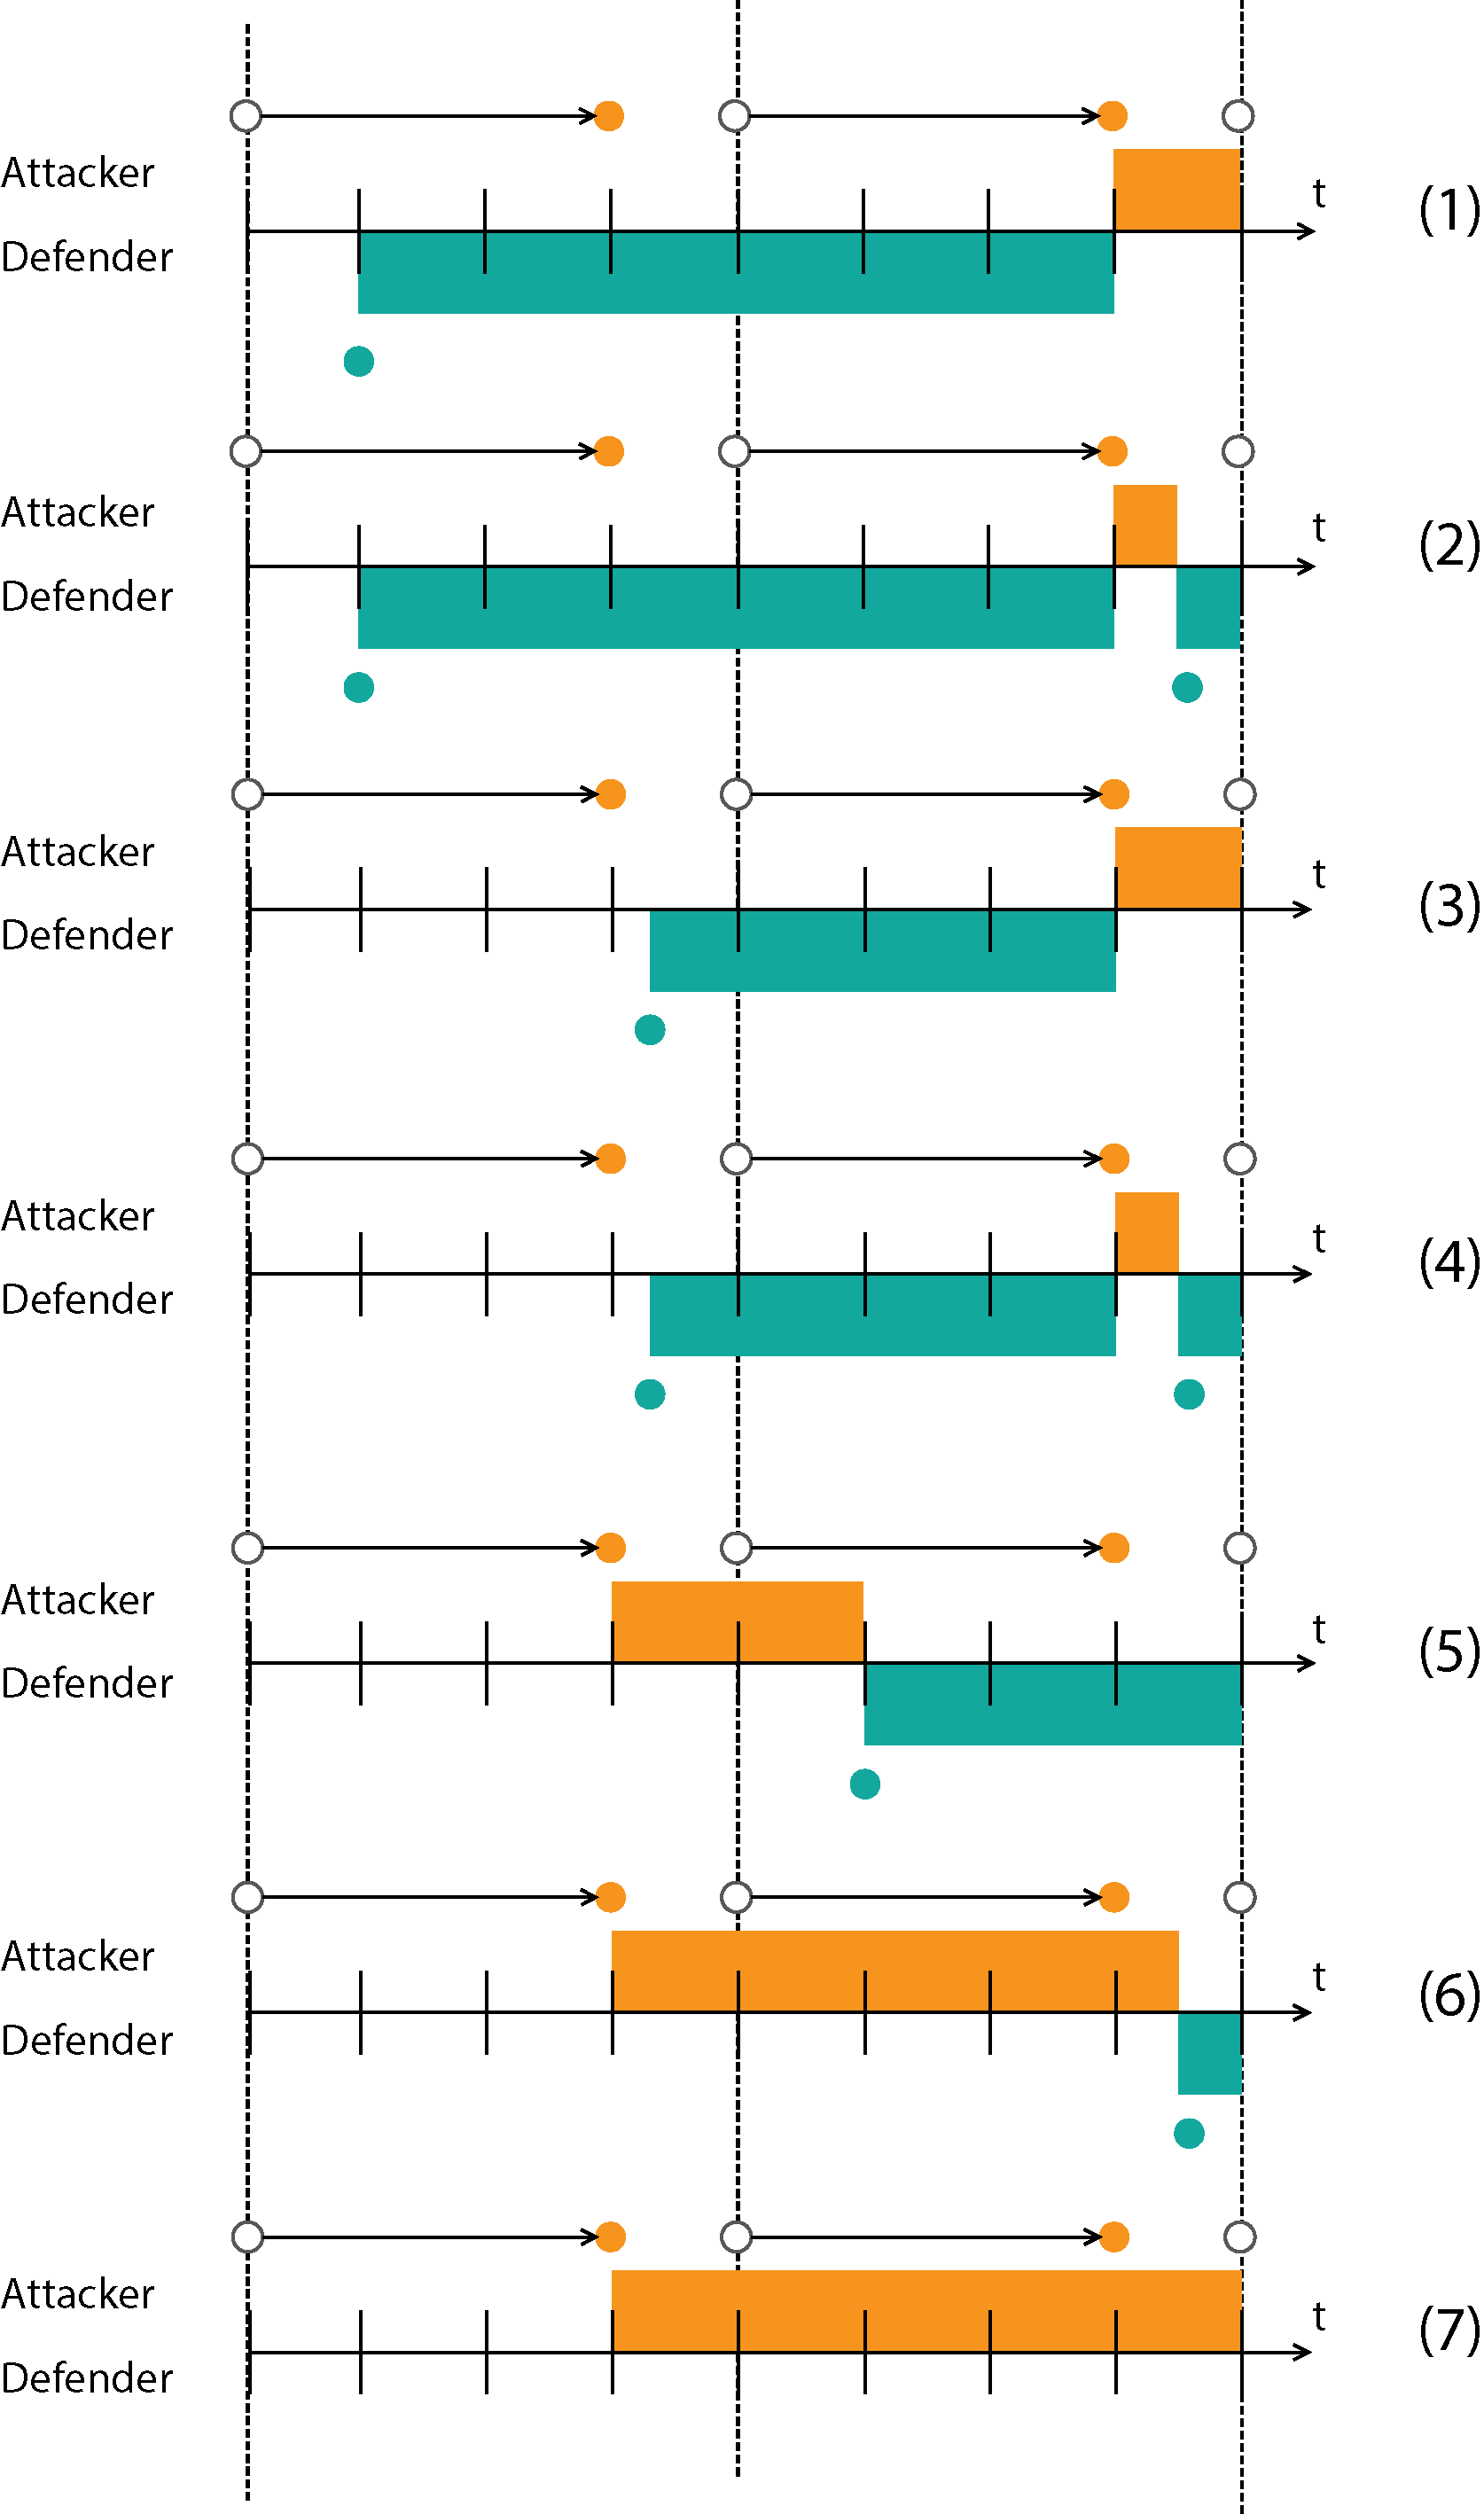
\includegraphics[scale=0.7]{../../doc/template/Images/FlipItCase2a.png}
\label{fig:case2}
\end{figure}


It is crucial that $ \delta_{D}$ is at least as large as $d + \delta_{A}$. If not, this would mean that the defender can move during the delay in the interval following the interval where the defender already moved. This would mean that there can be an overlap between the average gain of $\dfrac{\delta_{A}}{2}$ and the delay. The above benefit formula would then include to much gain for the defender: the potential overlap during the delay would be counted twice. \\


~~ \\
\subsubsection*{\textbf{Case b:} $d + \delta_{A} \geq \delta_{D}$}
~~~\\

To obtain the formula in case of a too long delay, we therefore need to subtract this overlapping gain from the above formula. 
Since $\delta_{D} \geq \delta_{A}$, if the defender enters the interval immediately after the attacker has played, then the defender cannot have played in the previous interval. In that case, there is no overlap. So the problem of the overlap only appears if the defenders enters late enough and thus only the last part of the delay is subject to overlap. The larger the difference between the interval of the defender and the attacker, the smaller the risk of overlap. Concretely, only the last part of length $d - (\delta_{D} - \delta_{A})$ is subject to overlap. Hence, the probability of overlap is $\dfrac{ d - (\delta_{D} - \delta_{A})}{\delta_{D}}$ and the gain will be half of this interval:  $\dfrac{ d - (\delta_{D} - \delta_{A})}{2}$.  The gain rate to be subtracted is therefore:\\

\begin{equation*}
\dfrac{1} {\delta_{A}} \cdot \dfrac{d - (\delta_{D} - \delta_{A})}{\delta_{D}} \cdot \dfrac{d - (\delta_{D} - \delta_{A})}{\delta_{D}}
\end{equation*}

The total gain  rate of the defender is obtained by subtracting this term from the gain rate of case a:
 \begin{equation*}
\gamma_{D}(\alpha_{D},\alpha_{A}) = \dfrac{\delta_{A}}{\delta_{D}} \cdot \dfrac{(d+\dfrac{\delta_{A}}{2})}{\delta_{A}} - \dfrac{(d - (\delta_{D} - \delta_{A}))^{2}}{2 \delta_{D} \delta_{A}}
\end{equation*}
\begin{equation*}
\gamma_{D}(\alpha_{D},\alpha_{A}) = \dfrac{\delta_{A}}{2\delta_{D}} + \dfrac{d}{\delta_{D}} - \dfrac{(d - (\delta_{D} - \delta_{A}))^{2}}{2 \delta_{D} \delta_{A}}
\end{equation*}\\
This yields in the following benefit formula:
\begin{equation*}
\beta_{D}(\alpha_{D},\alpha_{A}) = \dfrac{\delta_{A}}{2\delta_{D}} + \dfrac{d}{\delta_{D}} - k_{D} \alpha_{D} - \dfrac{(d - (\delta_{D} - \delta_{A}))^{2}}{2 \delta_{D} \delta_{A}}
\end{equation*}\\
 
The benefit for the attacker will be as follows:
\begin{equation*}
\beta_{A}(\alpha_{D},\alpha_{A}) = 1 -\dfrac{\delta_{A}}{2\delta_{D}} - \dfrac{d}{\delta_{D}} - k_{A} \alpha_{A} + \dfrac{(d - (\delta_{D} - \delta_{A}))^{2}}{2 \delta_{D} \delta_{A}}
\end{equation*}\\


